% Dokumentenklasse
\documentclass{article}

% Pakete
\usepackage{tex/pakete}
\usepackage{tex/macros}
\DeclareSIUnit\px{px}

% Einstellen der Pakete
\graphicspath{{figs/}}
\addbibresource{refs.bib}
\titleformat{\section}
  {\normalfont\LARGE\bfseries}{\thesection.}{.3em}{}
\titlespacing*{\section}{0pt}{3.5ex plus 1ex minus .2ex}{2.3ex plus .2ex}
\titleformat{\subsection}
  {\normalfont\Large\bfseries}{\thesubsection.}{.3em}{}
\titlespacing*{\subsection}{0pt}{3.5ex plus 1ex minus .2ex}{2.3ex plus .2ex}
\titleformat{\subsubsection}
  {\normalfont\large\bfseries}{\thesubsubsection.}{.3em}{}
\titlespacing*{\subsubsection}{0pt}{3.5ex plus 1ex minus .2ex}{2.3ex plus .2ex}

\sisetup{output-decimal-marker = {,}}

%\numberwithin{equation}{section}
%\counterwithin{figure}{section}

\pagestyle{fancy}
%\fancyhf{}
\lhead{P401 Elektronische Übergänge in Atomen}
\rhead{Gabriel Remiszewski und Christian Fischer}

% Titelblatt
\title{\textbf{Versuchsbericht} \\ \Large{\textbf{P401 Elektronische Übergänge}}}
\date{durchgeführt am 13/14.12.2023 \\ betreut von Valentin Jonas}
\author{Gabriel Remiszewski und Christian Fischer}

%========================================================================
\begin{document}

\begin{titlepage}
\maketitle
\thispagestyle{empty}
\end{titlepage}
\newpage
\tableofcontents
\thispagestyle{empty}
\newpage

% "Einleitung"
\section{Einleitung}\label{sec:einleitung}
\pagenumbering{arabic}
\cite{skript}

% "Versuchsabschnitte"
\section{Zeeman-Effekt}\label{sec:zeeman}
Der Zeeman-Effekt beschreibt die Aufspaltung der Energieniveaus einzelner Zustände 
in einem Magnetfeld. Spin und Bahndrehimpuls bewirken ein magnetisches Moment, auf welches 
ein äußere Magnetfeld wirken kann. Quantenmechanisch kann dies durch den Hamiltonoperator 
beschrieben werden, der die Interaktion mit einem äußeren Feld beschreibt \cite{Sakurai}:
\begin{equation}
    \hat H_\mathrm{int} = -\frac{q}{2m_\mathrm e}\qty(\hat{\vec L} + 2\hat{\vec S})\cdot \vec B.
    \label{eq:zeeman_hamilton}
\end{equation}

In diesem Versuch wird die Aufspaltung an Cadmium beobachtet. Das äußere Elektron sieht 
aufgrund der Wahrscheinlichkeitsverteilung in erster Näherung den Kern mit den inneren 
Schalen effektiv als nur ein Teilchen, womit die Berechnung der Energieniveaus 
äquivalent zum Wasserstoffatom betrachtet werden kann. Da dieses durch eine gerade 
Elektronenzahl keinen Gesamtspin 
besitzt und das Magnetfeld homogen ist, vereinfacht sich \cref{eq:zeeman_hamilton} zu 
\begin{equation*}
    \hat H_\mathrm{int} = \frac{eB}{2m_\mathrm e}\hat{L_z},
\end{equation*}
wobei die Elektronenladung eingesetzt wurde und das Magnetfeld per Konvention in die z-Achse zeigt.
Da bei kugelsymmetrischem Potenzial die z-Komponente des Drehimpulsoperators mit dem restlichen Hamiltonoperator
des Atoms kommutiert, ergibt sich eine Verschiebung des Energieniveaus von
\begin{equation*}
    \Delta E = \frac{e\hbar}{2m_\mathrm e}m_jB \equiv \mu_\mathrm B m_j B
    \label{eq:energy_zeeman}
\end{equation*}

mit dem Bohrschen Magneton \cite{Demtröder:829119}
\begin{equation}
    \mu_B = \SI{9.274015}{\joule\per\tesla}.
    \label{eq:magneton}
\end{equation}
Weil hier elektrische Dipolübergänge betrachtet werden, gilt die Auswahlregel 
$\Delta m = \{\pm 1, 0\}$ \cite{Demtröder:829119}, wobei einer Differenz 
von null linear polarisiertes Licht (im folgenden als $\pi$ bezeichnet) und einer Differenz von $\pm 1$
zirkular polarisiertes Licht ($\sigma^+$ für links zirkular und $\sigma^-$ für rechts zirkular) 
zugeordnet werden kann.
Für $\pi$-Polarisation kann daher keine Energieverschiebung beobachtet werden, für 
$\sigma^\pm$-Polarisation eine Verschiebung von 
\begin{equation}
    \delta E = \pm \mu_\mathrm B B
    \label{eq:normal_zeeman}.
\end{equation}
Unabhängig von der Drehimpulsquantenzahl kann somit beim hier beschriebenen 
normalen Zeeman-Effekt immer nur eine Aufspaltung in drei Linien beobachtet werden,
weshalb die Entartung nur teilweise aufgehoben werden kann.

In \cref{fig:zeeman_übergänge} ist das Übergangsschema für die Übergänge ${}^1D_2\rightarrow {}^1P_1$
des Cadmiumatoms dargestellt. Die Wellenlänge des Übergangs ist $\lambda_0 = \SI{644}{\nano\meter}$
und entspricht rotem Licht. Dieser Übergang wird in diesem Versuch untersucht.

\begin{figure}
    \centering
    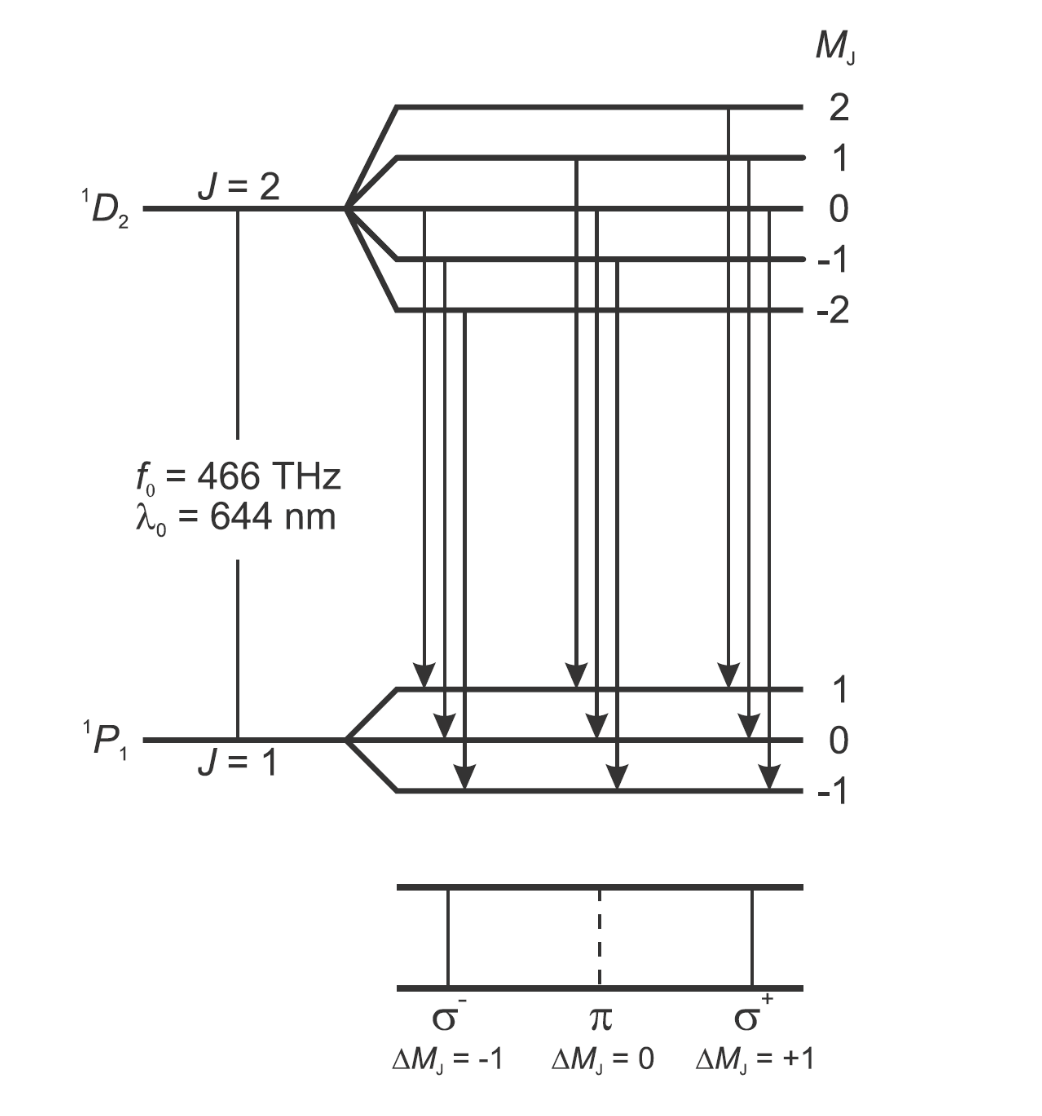
\includegraphics[width=0.6\linewidth]{../figs/zeeman_übergänge}
    \caption{Übergangsschema von Cadmium für die Singulett-Zustände ${}^1D_2\rightarrow {}^1P_1$. 
        Zusehen sind jeweils drei Übergangsgruppen mit je drei Übergängen, die untereinander
        entartet sind, die Entartung zwischen einander jedoch durch den Zeeman-Effekt aufgehoben wird. Darunter 
        ist die durch die Auswahlregeln bestimmte Polarisation des abgestrahlten Lichts aufgetragen. 
        \cite{zeeman_handblatt}}
    \label{fig:zeeman_übergänge}
\end{figure}

\subsection{Versuchsaufbau}
Der Aufbau zur Untersuchung des Zeeman-Effekts ist in \cref{fig:zeeman_aufbau} skizziert. Eine 
Cadmiumlampe wird zwischen ein Magnetfeld festgehalten, welches durch zwei in Reihe 
geschalteten stromdurchflossenen Spulen erzeugt wird. Die Spulen können 
um die vertikale Achse gedreht werden, um die Richtung 
des Magnetfeldes in Bezug zur Beobachtungsrichtung verändern zu können. 
Das Licht der Lampe wird mit einer Kondensorlinse 
$f=\SI{150}{\mm}$ kollimiert mit leichter Konvergenz, um nachher am Etalon verschieden Einfallswinkel zu 
erzeugen. 

Das eingebaute Fabry-P\'erot-Etalon ist eine planparallele Glasschicht, welche 
beidseitig mit teildurchlässigen Spiegeln beschichtet ist. Durch ständige Reflexion innerhalb der Glasschicht
wird ein Strahlenbündel erzeugt, welches durch Gangunterschiede untereinander interferiert. 
Das hier benutzte Etalon hat einen Brechungsindex von $n=1.457$ und einem Reflexionsgrad $R=0.85$.
Mit einer weiteren Sammellinse $f=\SI{150}{\mm}$ wird das Licht am Okular scharf abgebildet, an 
dem durch die entstandene Interferenz konzentrische Ringe Beobachter sein können. Davor wird mit einem 
Interferenzfilter das rote Licht bei $\SI{644}{\nm}$ gefiltert.

\begin{figure}[h]
    \centering
    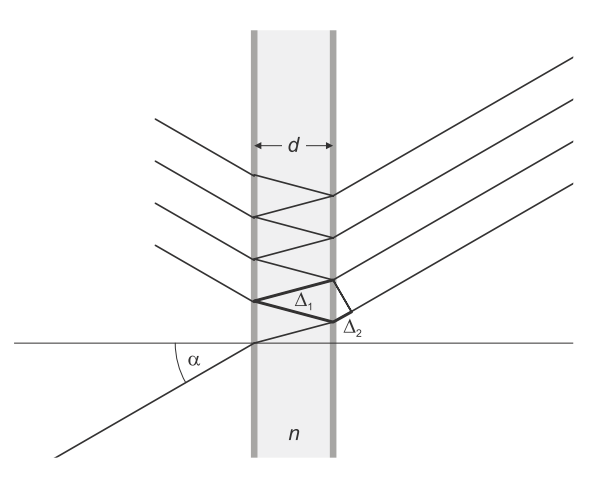
\includegraphics[width=0.6\linewidth]{../figs/etalon}
    \caption{Funktionsweise eines Fabry-P\'erot-Etalon. $\alpha$ bezeichnet den Einfallswinkel 
        eines Lichtstrahls in den Etalon mit Dicke $d$ bei Brechungsindex $n$.
        $\Delta_1$ und $\Delta_2$ bezeichnen die Gangunterschiede, die zur Interferenz zweier 
        transmittierter Strahlen führen.
        \cite{zeeman_handblatt}}
    \label{fig:etalon}
\end{figure}

\begin{figure}[h]
    \centering
    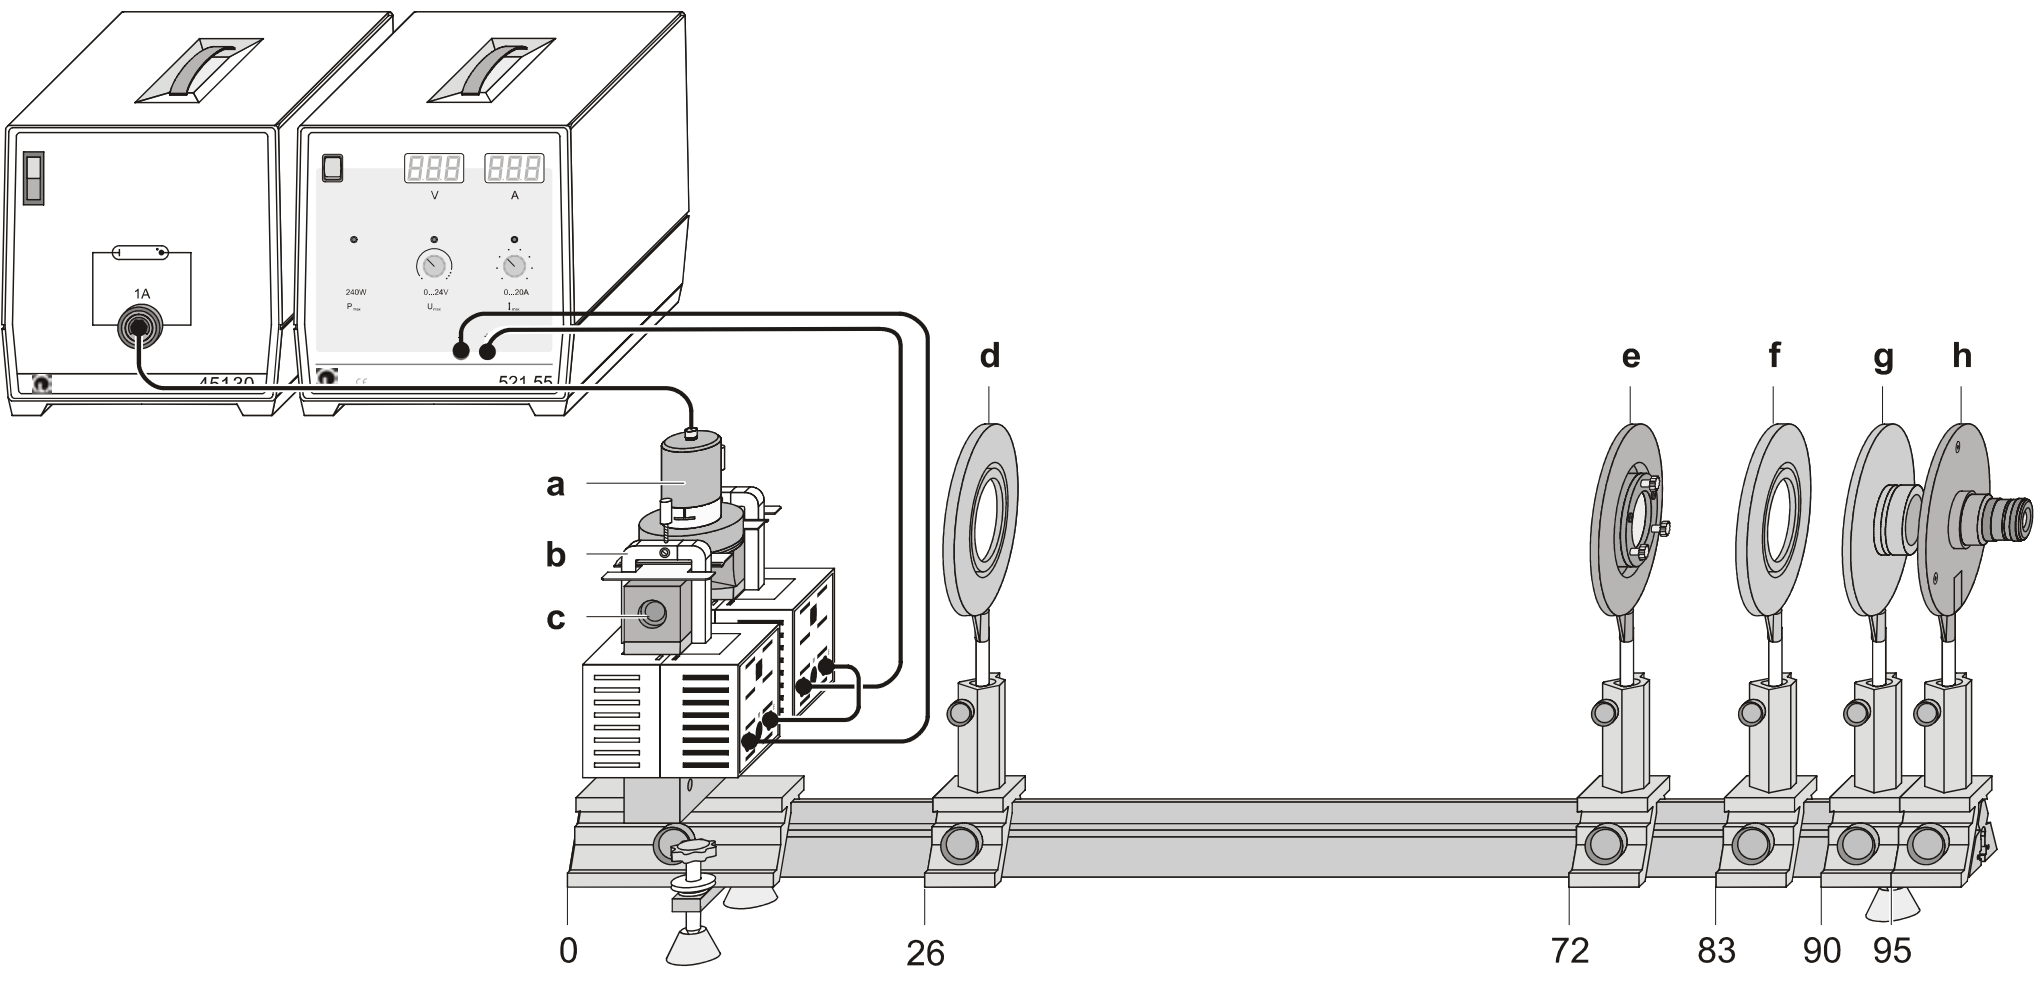
\includegraphics[width=0.7\linewidth]{../figs/zeeman_aufbau}
    \caption{Aufbau zur Messung des Zeeman-Effekts. \abf a zeigt die Cadmiumlampe mit Klammern
        \abf b und Polschuhe \abf c. \abf d zeigt die Kondensorlinse, \abf e das Etalon, \abf f 
        die Abbildungslinse, \abf g das Interferenzfilter und \abf h das Okular mit Strichskala. 
        \cite{zeeman_handblatt}}
    \label{fig:zeeman_aufbau}
\end{figure}

\subsection{Untersuchung der Transversal- und Longitudinalkonfiguration}\label{sec:zeeman_quantitativ}
Durch das Drehen der Spulen lässt sich die Polarisation der emittierten Strahlung 
untersuchen. Hierbei werden zwei Konfigurationsmöglichkeiten gesondert betrachtet.
Klassisch lässt sich die Polarisations- und Strahlrichtung der Übergangsstrahlung 
mit dem Lorentz-Modell beschreiben, wo eine Schwingungsgleichung mit der Lorentzkraft als 
treibende Kraft angesehen wird. Dabei sind $\pi$- und $\sigma^\pm$-Strahlung die Eigenmodi 
der Lösung. Diese sind in \cref{fig:zeeman_polarisation} skizziert. Zu sehen ist hierbei, 
dass sich jede Lösung als schwingender Dipol interpretieren lässt, wobei für $\sigma^\pm$ 
zwei senkrecht zueinander stehenden Dipole mit einer $\SI{90}{\degree}$-Phasenbeziehung 
betrachtet werden.

Da Dipole nicht in Bewegungsrichtung abstrahlen, kann in longitudinaler 
Beobachtungsrichtung (parallel zum Magnetfeld) nur die zirkular polarisierte $\sigma^\pm$-Strahlung
beobachtet werden. Bei transversaler Konfiguration sind alle drei Modi sichtbar mit dem 
Unterschied, dass $\sigma^\pm$ hier linear polarisiert ist und räumlich um $\SI{90}{\degree}$
zur $\pi$-Polarisation gedreht.

\subsubsection{Transversalkonfiguration}
In Transversalrichtung können $\sigma^\pm$- sowie $\pi$-Strahlung beobachtet werden, wobei 
diese Modi linear polarisiert sind und senkrecht zueinander stehen. Mit einem Polarisationsfilter 
lässt sich somit $\pi$ und $\sigma$ voneinander trennen, $\sigma^+$ und $\sigma^-$ sind jedoch nicht 
unterscheidbar voneinander. Vor das Etalon wird der Polarisationsfilter befestigt und 
beim Einschalten des Magnetfeldes das Bild beobachtet. Die optische Achse 
des Filters steht auf $\SI{0}{\degree}$, wenn Diese senkrecht zur optischen Bank
steht. Erwartet wird das Verschwinden der inneren Ringe bei einer Filterausrichtung von 
\SI{0}{\degree}, da in diesem Falle die optische Achse des Filters senkrecht zum B-Feld und damit 
zur Polarisationsachse des $\pi$-Lichts steht. Damit ist das Verschwinden der äußeren Ringe 
bei \SI{90}{\degree} zu erwarten.

In \cref{fig:transversal_konfiguration} sind die Interferenzringe abgebildet. Durch das Anlegen
eines Magnetfeldes wurde die Aufspaltung der Ringe in einen hellen mittleren 
Ring und zwei leicht dunklere daneben deutlich. Aufgrund des Auflösungsvermögens und möglicherweise 
einer Überbelichtung konnten die Details des Bildes auf der Aufnahme nicht kenntlich
gemacht werden. Bei einer Polarisationsfiltereinstellung von \SI{0}{\degree} verschwinden
die inneren Ringen, bei \SI{90}{\degree} die Äußeren. Dies entspricht dem erwarteten Verhalten, 
weshalb daraus geschlossen werden kann, dass das Licht der äußeren Ringe senkrecht zum 
B-Feld polarisiert ist und das Licht der inneren Ringe parallel dazu.

\begin{figure}[h]
    \centering
    \begin{subfigure}{0.45\linewidth}
        \centering
        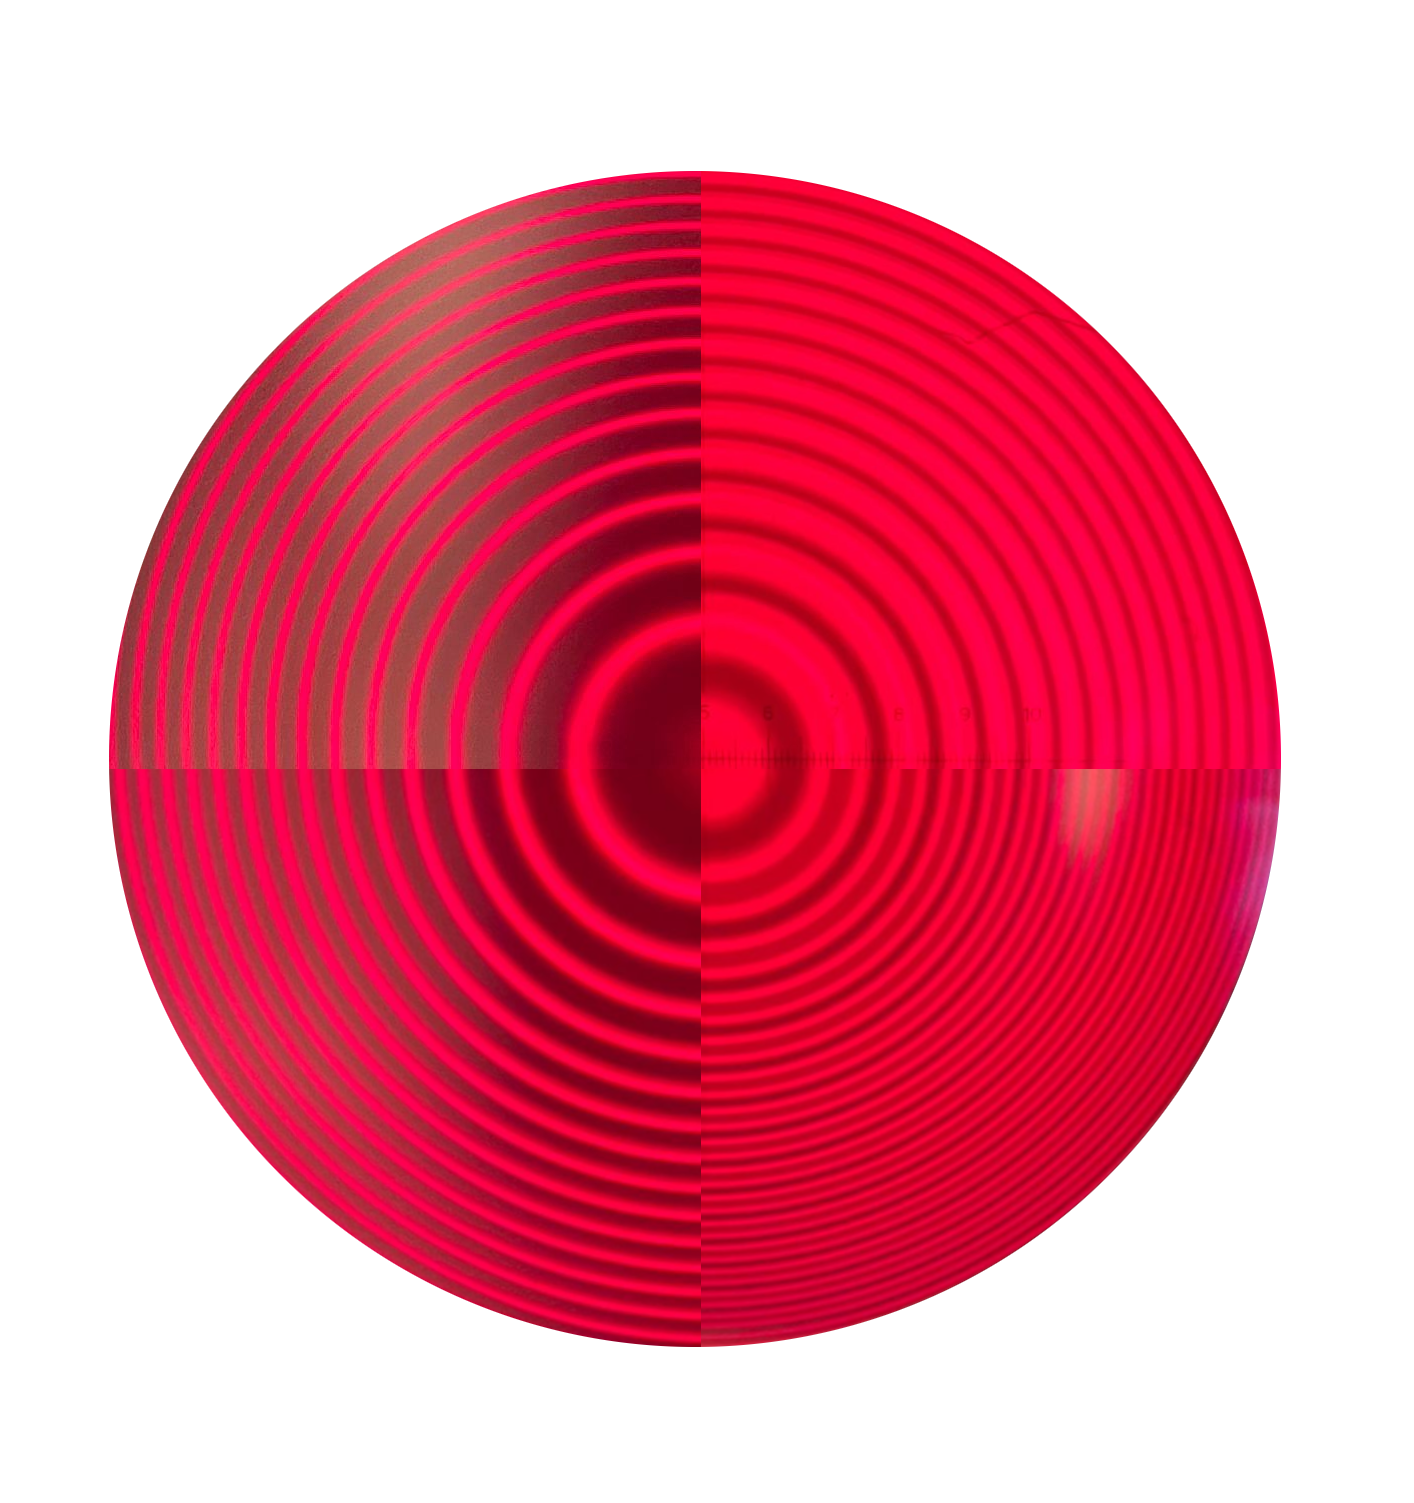
\includegraphics[width=\linewidth]{../figs/transversal_konfig}
        \caption{Transversal Konfiguration: links oben ohne B-Feld, rechts oben mit B-Feld,
            rechts unten mit Filter auf $\SI{0}{\degree}$, links unten mit Filter auf $\SI{90}{\degree}$.}
        \label{fig:transversal_konfiguration}
    \end{subfigure}
    \hspace{.5cm}
    \begin{subfigure}{0.45\linewidth}
        \centering
        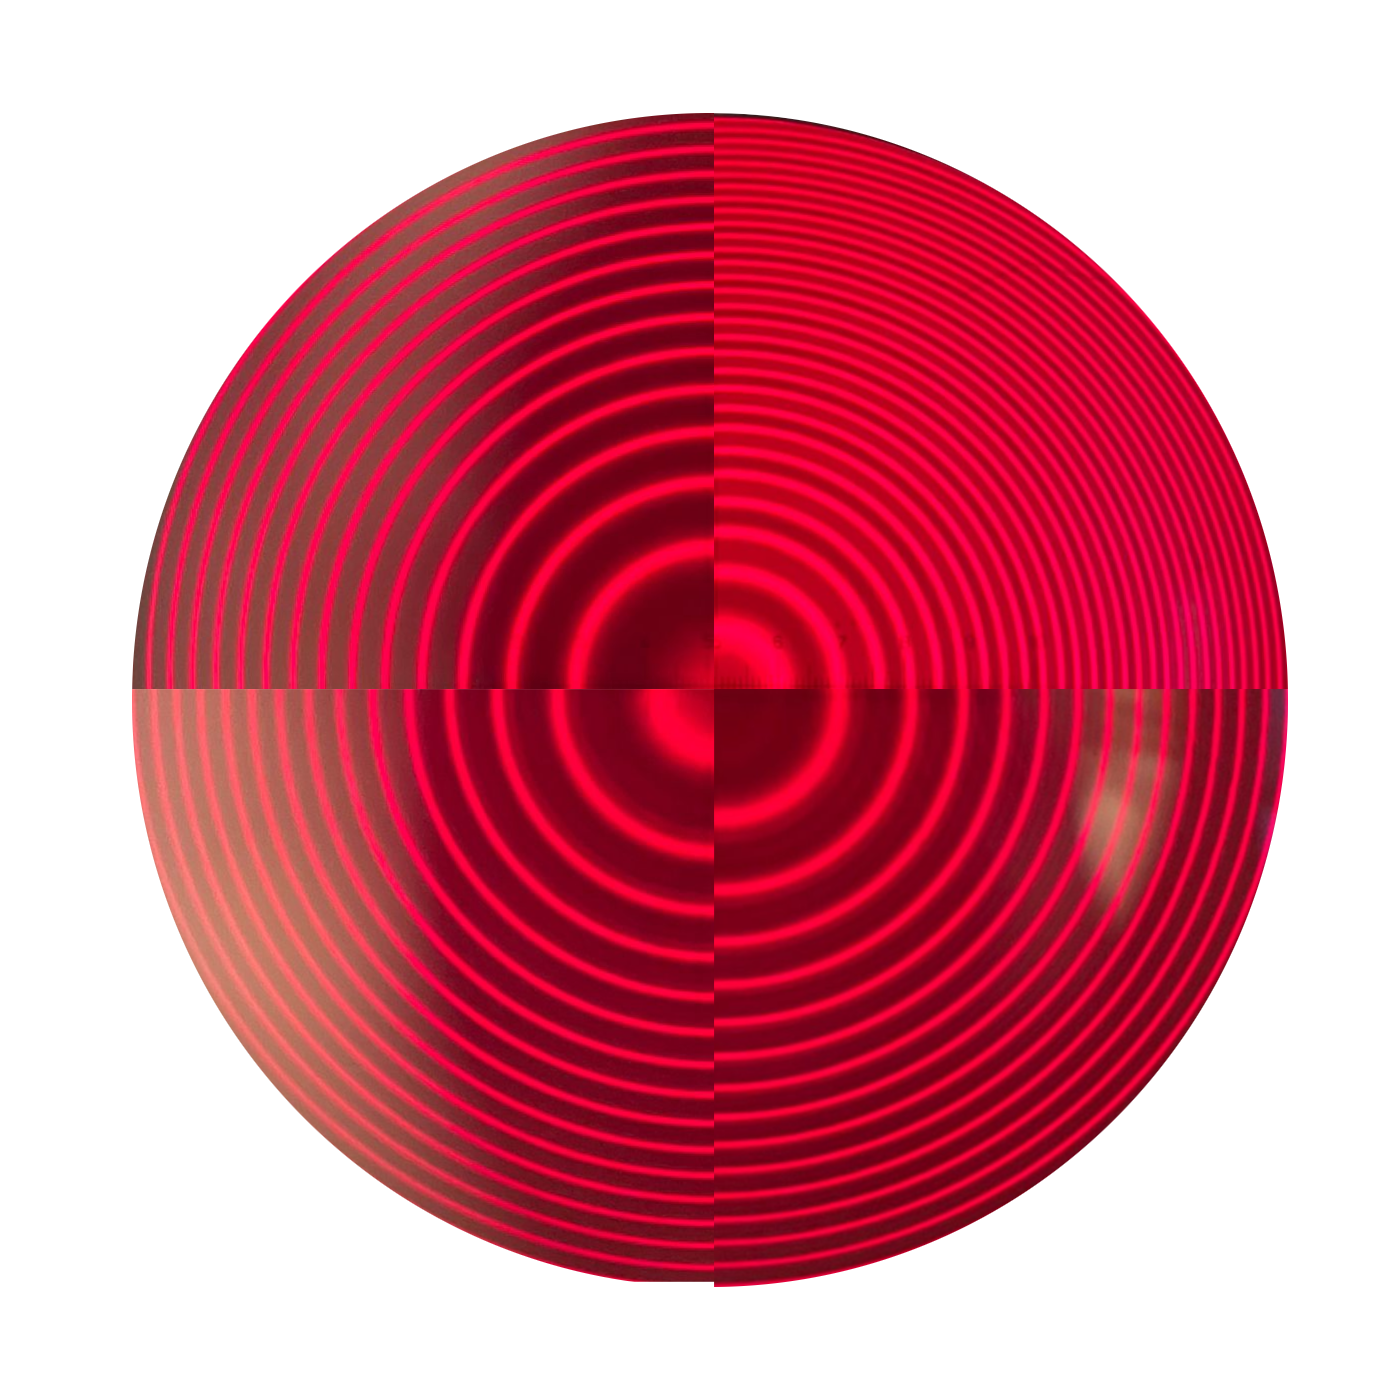
\includegraphics[width=\linewidth]{../figs/longitudinal_konfig}
        \caption{Longitudinal Konfiguration: links oben ohne B-Feld, rechts oben mit B-Feld, 
        rechts unten mit Filter auf $\SI{+45}{\degree}$, links unten mit Filter auf $\SI{-45}{\degree}$. }
        \label{fig:longitudinal_konfiguration}
    \end{subfigure}
    \caption{Aufnahmen der Etalon Interferenzringe bei unterschiedlichen Aufbauten.}
\end{figure}


\subsubsection{Longitudinalkonfiguration}
In longitudinaler Ausrichtung kann nur das $\sigma^\pm$-Licht beobachtet werden. Um zu zeigen, 
dass beide Wellen zirkular und entgegengesetzt polarisiert sind, wird vor dem Polarisationsfilter 
eine $\lambda/4$-Wellenplatte befestigt, welche die Phase des elektrischen Feldes parallel 
zur optischen Achse um eine viertel Wellenlänge verschiebt und somit zirkulares Licht 
linear polarisieren kann. Per Definition entsprechen $\sigma^\pm$ die komplexen Vektoren des 
elektrischen Feldes 
$\vb E_\mathrm{\sigma^\mp} \propto \vb e_x \mp i\vb e_y$. Ohne Beschränkung der Allgemeinheit wird die optische Achse 
der Wellenplatte auf die y-Achse gesetzt. Bei einer Verzögerung wird die y-Komponente 
um den Faktor $\e^{\pm i\pi /2} = \pm i$ verschoben, womit sich eine Polarisation von 
$\vb E_\mathrm{\sigma^\mp}\propto \vb e_x \pm \vb e_y$ ergibt. Somit ist $\sigma^-$ 
bei einer Ausrichtung des Filters bei \SI{45}{\degree} sichtbar, während $\sigma^+$ Licht 
bei \SI{-45}{\degree} sichtbar wird. 

In \cref{fig:longitudinal_konfiguration} ist die Longitudinalkonfiguration gezeigt. Es ist zu erkennen,
das sich diesmal beim Anlegen eines Magnetfeldes die Linie in nur zwei symmetrisch verteilte Linien 
aufspaltet. Nach Durchgang einer Verzögerungsplatte und einer Filtereinstellung von $\pm\SI{45}{\degree}$
verschwindet wie erwartet jeweils einer der zwei Ringe. Aufgrund der oberen Überlegung 
lässt sich damit der innere Ring $\sigma^-$-Licht zuweisen und $\sigma^+$-Licht dem äußeren Ring.
Auf die Relation, dass $\sigma^-$ kleinere Winkel und $\sigma^+$ größere Winkel zuzuordnen sind, wird 
bei der Bestimmung des Bohr Magnetons weiter eingegangen.


\begin{figure}[htb]
    \centering
    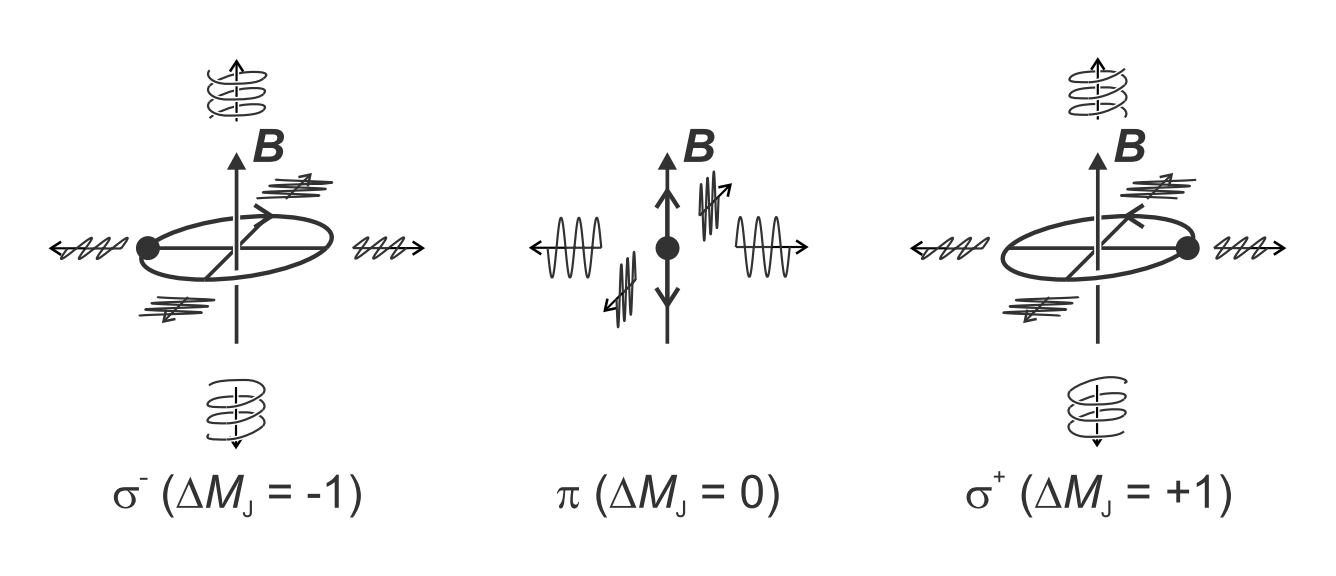
\includegraphics[width=0.6\linewidth]{../figs/zeeman_polarisation}
    \caption{Polarisation der verschiedenen Übergänge. $\pi$-Strahlung ist nur in transversaler 
    Richtung beobachtbar, $\sigma^\pm$-Strahlung in transversaler und in longitudinaler 
    Richtung. \cite{zeeman_handblatt}}
    \label{fig:zeeman_polarisation}
\end{figure}

\subsection{Bestimmung des Bohrschen Magnetons}\label{sec:magneton}
Zur Bestimmung des Bohrschen Magnetons wird die Aufspaltung der Linien 
in Transversalkonfiguration mit einer CCD-Kamera gemessen. Diese Messung wird 
bei unterschiedlichen Spulenströmen 40-mal durchgeführt und der Mittelwert 
gespeichert für genauere Ergebnisse. Mit einer Hall-Sonde wird 
zur Kalibration das Magnetfeld in Abhängigkeit des Stroms vor und nach der Durchführung
einer Messung vorgenommen. Durch das Erhitzen der Spulen wird erwartet, dass sich 
die Kalibrationskurve mit der Zeit ändert. Durch zwei Messungen kann damit der Fehler des 
Magnetfeldes bestimmt werden.

Untersucht wird hierbei ein einzelnes Interferenzmaximum nahe des Ringzentrums. Dieses wird 
beim Anlegen eines Magnetfeldes in drei Maxima aufgespalten. An die gemessenen Kurven 
werden drei Gauss-Kurven mit einem linearen Offset angepasst. Die Anpassfunktion kann somit beschrieben werden 
mit 
\begin{equation*}
    f(x, \vec x, \vec \sigma, \vec A, m, n) = \sum_{i=1}^3 \frac{A_i}{\sqrt{2\pi}\sigma_i}
        \exp\qty(-\frac{(x-x_i)^2}{2\sigma_i^2}) +mx + n.
\end{equation*}

Das Programm zur Messung der Einstrahlintensitäten gibt keine dazugehörigen Unsicherheiten an.
Aus diesem Grund müssen diese rekonstruiert werden. Die CCD-Kamera misst Photonen, wodurch 
die Messung pro Pixel als Poisson-verteilt angesehen werden kann mit dazugehörigem Poisson-Fehler \\
$\Delta N = \sqrt{N}$. Die Umrechnung der Zählereignisse in eine Intensität (in Prozent) ist unbekannt, 
weshalb der Fehler mit einem unbekannten Faktor skaliert wird. Für die Anpassungskurve 
ist dieser jedoch irrelevant, da nur der relative Fehler der einzelnen Messpunkte von Bedeutung ist. 
Der Skalierungsfaktor ist daher nicht nötig. Da jedoch nur die relativen Fehler bekannt sind, verliert 
die Berechnung einer Anpassungsgüte, wie dem reduzierten Chi-Quadrat \cite{wiki:reduced_chi_square},
seine Bedeutung, weshalb eine quantitative Bewertung der Anpassungen nicht durchgeführt werden kann.

\begin{figure}
    \centering
    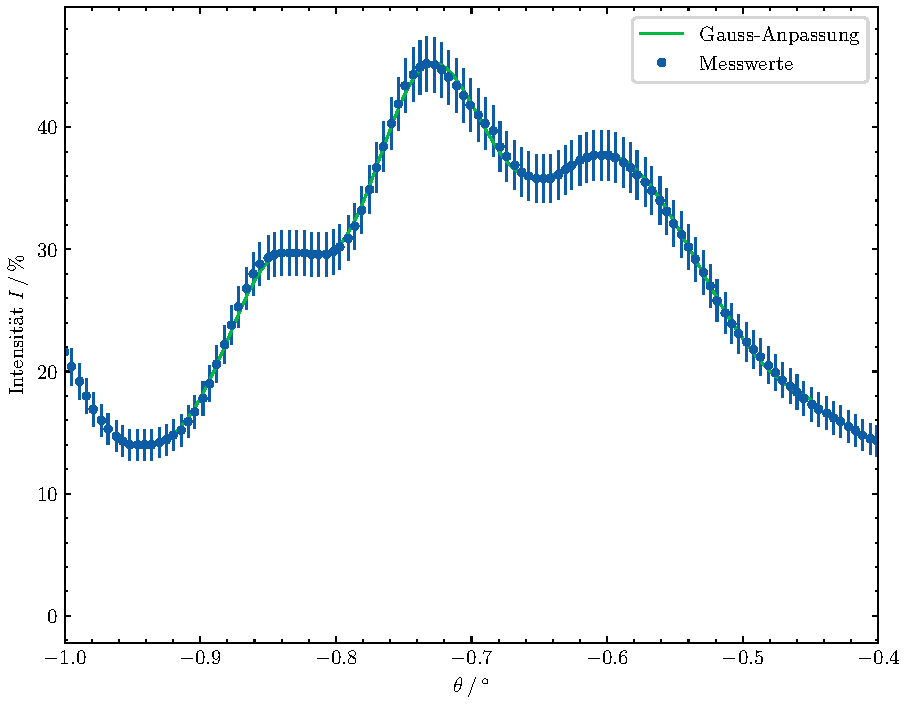
\includegraphics[width=.6\linewidth]{../figs/gauss_i7.9.pdf}
    \caption{Aufspaltung der Maxima bei einem Strom von \SI{7.9}{\ampere}.}
    \label{fig:gauss_i79}
\end{figure}

Eine Anpassungskurve ist beispielhaft in \cref{fig:gauss_i79} gezeigt. Visuell
kann die Anpassung als äußerst erfolgreich angesehen werden. Weitere Diagramme 
sind im \cref{sec:anhang} zu finden.

Die Mittelwerte und Standardabweichungen der Gauß-Kurven sind tabellarisch in \cref{tab:gauss_zeeman_maxima_and_std}
dargestellt. Es fällt auch, dass das mittlere Maximum nicht immer am gleichen Winkel vorzufinden ist. Daraus lässt sich 
schließen, dass während der Messung der Mittelpunkt der Ringe stets in einem kleinen Bereich geschwankt 
ist. Der daraus resultieren Fehler wird für kleine Winkel 
jedoch nur linear mit der Verschiebung ansteigen und im Vergleich zu anderen Fehlern gering sein.
Mit \cref{fig:etalon} lässt sich für die Maxima die Bedingung 
\begin{equation}
    \lambda = \frac{2d}{m}\sqrt{n^2-\sin^2\alpha}, \qquad 
    \Delta\lambda \approx = \frac{2d}{m}\frac{\alpha \Delta\alpha}{\sqrt{n^2 - \alpha^2}}
    \label{eq:etalon_gleichung}
\end{equation}
mit der Beugungsordnung $m$ herleiten. Für die Unsicherheit wurde die Kleinwinkelnäherung benutzt, was 
hier keinen Unterschied machen sollte, da diese sowieso auf die erste oder zweite signifikante Stelle
aufgerundet werden.
Mit \cref{eq:etalon_gleichung} und dem mittleren Maximum bei bekannter Wellenlänge von \SI{644}{\nm}
lässt sich die Beugungsordnung bestimmen. Diese lag beim untersuchten Maximum bei 
$m = \num{18104}$.

Im Folgenden wird die Wellenlängendifferenz eines äußeren und dem mittleren Maximum als 
\\$\delta\lambda = \lambda_{\sigma^\pm} - \lambda_\pi$ definiert. Damit ist die 
Energieverschiebung gegeben mit 
\begin{equation*}
    \delta E = hc\qty(\frac{1}{\lambda_{\sigma^\pm}} - \frac{1}{\lambda_\pi})
        \equiv -E_0\frac{\delta\lambda}{\lambda_\pi+\delta\lambda}
\end{equation*}

Aufgrund von \cref{eq:etalon_gleichung} lässt sich sagen, das im betrachteten Bereich 
die Wellenlänge steigen muss bei kleineren Winkeln. Da eine höhere Wellenlänge zu kleineren 
Energien führt, führen kleinere Winkel zu kleineren Energien. Damit also 
$\delta E_{\sigma^\pm} = \pm \mu_\mathrm B B$ ist, muss $|\alpha_{\sigma^+}| > |\alpha_0|$
und $\abs{\alpha_{\sigma^-}} < \abs{\alpha_0}$ sein. Aus diesem Grund 
lässt sich das rechte Maximum (innerer Ring) $\sigma^-$ und das linke Minimum 
(äußerer Ring) $\sigma^+$ zuweisen, da negative Winkel betrachtet wurden. Dies stimmt mit 
den Überlegungen in \cref{sec:zeeman_quantitativ} überein.

\begin{figure}[htb]
    \centering
    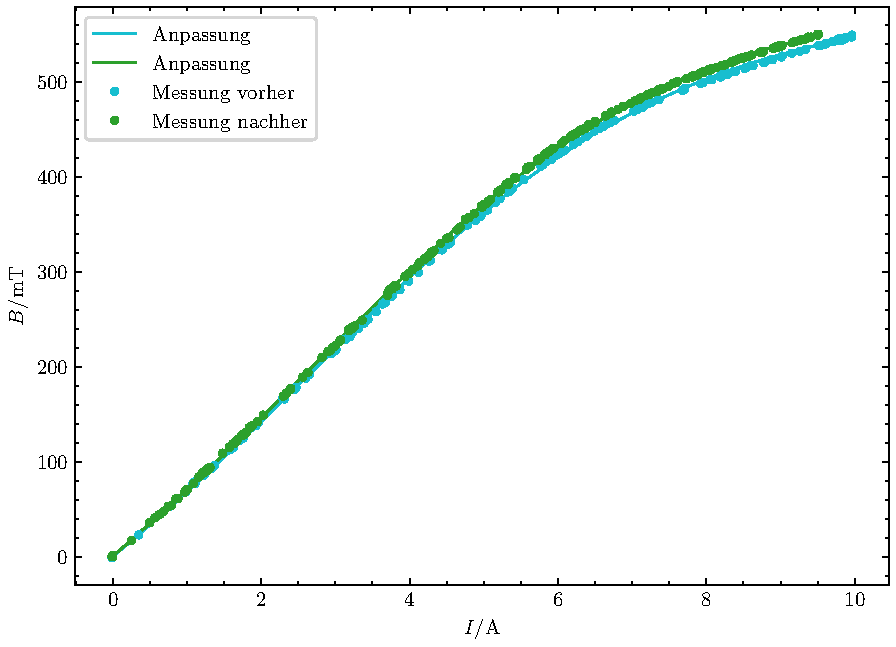
\includegraphics[width=.6\linewidth]{../figs/BFeld-Kalibrationskurve}
    \caption{Magnetfeldkalibration}
    \label{fig:bfield_kalibration}
\end{figure}

Um das Magneton zu bestimmen muss noch die Magnetfeldkalibration durchgeführt werden. 
Hierfür wird an die Messdaten der Hall Sonde vor und nach der Messung der Interferenzringe 
die Funktion 
\begin{equation*}
    B(I) = \alpha + \frac{\beta}{(\gamma + \e^{-\delta I})^\varepsilon}
\end{equation*}

angepasst.

\begin{table}[h]
   \centering
\caption{Anpassparameter der Magnetfeldkalibration}
\begin{tabular}{c c c c c c c}
\hline Magnetfeldmessung & $\alpha / \unit{\milli\tesla}$ & $\beta / \unit{\milli\tesla}$ & $\gamma$ & $\delta$ & $\epsilon$ & $\chi^2$ \\ 
\hline
vorher & $\num{-1140\pm 120}$ & $\num{1150\pm 120}$ & $\num{0.022\pm 0.003}$ & $\num{0.621\pm 0.014}$ & $\num{0.092\pm 0.011}$ & $\num{7.15}$ \\
nachher & $\num{-1100\pm 70}$ & $\num{1100\pm 70}$ & $\num{0.0097\pm 0.0012}$ & $\num{0.748\pm 0.015}$ & $\num{0.074\pm 0.006}$ & $\num{1.89}$ \\
\hline\end{tabular}
\label{fig:kalibration_tabelle}
\end{table}

\begin{table}[htbp]
   \centering
\caption{Maxima und Standardabweichungen der Gauss-Anpassungen}
\begin{tabular}{c c c c c c c}
\hline$I / \unit{\ampere}$ & $x_\mathrm{links} / \unit{\degree}$ & $x_\mathrm{mitte} / \unit{\degree}$ & $x_\mathrm{rechts} / \unit{\degree}$ & $\sigma_\mathrm{links} / \unit{\degree}$ & $\sigma_\mathrm{mitte} / \unit{\degree}$ & $\sigma_\mathrm{rechts} / \unit{\degree}$ \\ 
\hline
$\num{4.7}$ & $\num{-0.8253\pm 0.0013}$ & $\num{-0.7481\pm 0.0011}$ & $\num{-0.6590\pm 0.0018}$ & $\num{0.0292\pm 0.0009}$ & $\num{0.0337\pm 0.0012}$ & $\num{0.076\pm 0.003}$ \\
$\num{5.2}$ & $\num{-0.8288\pm 0.0015}$ & $\num{-0.7438\pm 0.0009}$ & $\num{-0.6394\pm 0.0017}$ & $\num{0.0306\pm 0.0012}$ & $\num{0.0384\pm 0.0014}$ & $\num{0.065\pm 0.003}$ \\
$\num{5.7}$ & $\num{-0.8392\pm 0.0009}$ & $\num{-0.7518\pm 0.0007}$ & $\num{-0.6443\pm 0.0009}$ & $\num{0.033\pm 0.001}$ & $\num{0.0375\pm 0.0008}$ & $\num{0.0689\pm 0.0014}$ \\
$\num{6.0}$ & $\num{-0.839\pm 0.003}$ & $\num{-0.750\pm 0.002}$ & $\num{-0.643\pm 0.003}$ & $\num{0.036\pm 0.004}$ & $\num{0.036\pm 0.002}$ & $\num{0.071\pm 0.005}$ \\
$\num{6.3}$ & $\num{-0.8455\pm 0.0009}$ & $\num{-0.7491\pm 0.0006}$ & $\num{-0.631\pm 0.001}$ & $\num{0.0339\pm 0.0012}$ & $\num{0.0411\pm 0.0008}$ & $\num{0.0642\pm 0.0015}$ \\
$\num{6.7}$ & $\num{-0.8417\pm 0.0009}$ & $\num{-0.7398\pm 0.0007}$ & $\num{-0.617\pm 0.001}$ & $\num{0.0338\pm 0.0011}$ & $\num{0.0428\pm 0.0009}$ & $\num{0.0605\pm 0.0018}$ \\
$\num{7.0}$ & $\num{-0.846\pm 0.003}$ & $\num{-0.742\pm 0.003}$ & $\num{-0.621\pm 0.004}$ & $\num{0.038\pm 0.006}$ & $\num{0.042\pm 0.003}$ & $\num{0.059\pm 0.006}$ \\
$\num{7.3}$ & $\num{-0.850\pm 0.001}$ & $\num{-0.7421\pm 0.0008}$ & $\num{-0.6150\pm 0.0012}$ & $\num{0.0358\pm 0.0017}$ & $\num{0.0443\pm 0.0011}$ & $\num{0.059\pm 0.002}$ \\
$\num{7.8}$ & $\num{-0.8489\pm 0.0013}$ & $\num{-0.738\pm 0.001}$ & $\num{-0.6050\pm 0.0015}$ & $\num{0.036\pm 0.003}$ & $\num{0.0452\pm 0.0013}$ & $\num{0.061\pm 0.003}$ \\
$\num{7.9}$ & $\num{-0.8451\pm 0.0012}$ & $\num{-0.735\pm 0.001}$ & $\num{-0.5992\pm 0.0014}$ & $\num{0.0355\pm 0.0017}$ & $\num{0.0444\pm 0.0012}$ & $\num{0.0646\pm 0.0019}$ \\
\hline\end{tabular}
\label{tab:gauss_zeeman_maxima_and_std}
\end{table}
\section{Franck-Hertz-Versuch}\label{sec:franck-hertz}
Der Franck-Hertz-Versuch hat historisch maßgeblich zur Entwicklung 
der Quantenmechanik beigetragen und das damals von Niels Bohr vorgestellte 
Atommodell gestützt. Hierbei werden in einer Röhre Elektronen zu einer Anode hin 
beschleunigt und erzeugen einen messbaren 
Strom. Besitzen diese genügend kinetische Energie, so können 
diese inelastisch mit den Quecksilberatomen in dem Röhrengas stoßen, 
wobei der Energieübertrag zur Anregung atomarer Übergänge genutzt wird. 
Aufgrund der verringerten kinetischen Energie der beschleunigten Elektronen 
kommt es zu einem Stromeinbruch. Die dabei entstehende Spannungskurve wird 
wie in \cref{fig:franck-hertz-spannungskurve} erwartet. Die Stöße der Elektronen 
mit den Atomen ist ein statistischer Prozess. Ebenso unterliegt die Elektronengeschwindigkeit
einer Maxwell-Boltzmann-Verteilung, weshalb keine scharfen Maxima 
bei den entsprechenden Beschleunigungsspannungen erwartet werden, sondern 
normalverteilte Kurven.

Aus der Differenz den Abständen der Maxima kann somit die 
Energie des Übergangs bestimmt werden. Primär kann 
aufgrund des deutlich höheren Wirkungsquerschnittes der Übergang
${}6^1\mathrm S_0\rightarrow 6^3\mathrm P_1$ betrachtet werden. Der Wirkungsquerschnitt ist 
hierbei antiproportional zur freien Weglänge des Gases korreliert. 


\begin{figure}[h]
    \centering
    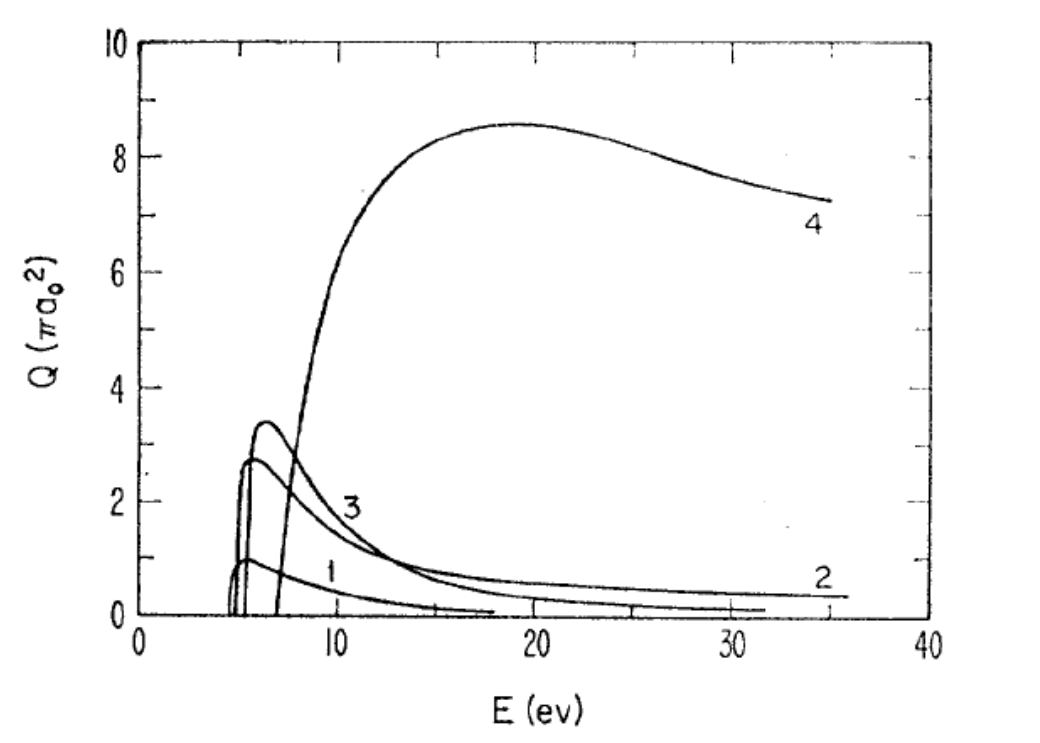
\includegraphics[width=0.6\linewidth]{../figs/querschnitt}
    \caption{Totale Wirkungsquerschnitte von \bf 1: $6^1\mathrm S_0\rightarrow 6^3\mathrm P_0$,
    \bf 2: $6^1\mathrm S_0\rightarrow 6^3\mathrm P_1$, 
    \bf 3: $6^1\mathrm S_0\rightarrow 6^3\mathrm P_2$,\\
    \bf 4: $6^1\mathrm S_0\rightarrow 6^1\mathrm P_1$ \cite{skript}}
    \label{fig:wirkungsquerschnitte}
\end{figure}

\subsection{Aufbau und Durchführung}
Um zunächst in einem Quecksilbergas freie Ladungsträger zu erzeugen, wird mit einer 
Heizspannung $U_\mathrm h$ ein Glühdraht erwärmt. In \cref{fig:schaltbild_franck_hertz} 
entspricht dies der Kathode K. Die Elektronen werden mit einer angelegten Beschleunigungsspannung
$U_\mathrm B$ zu einem Gitter G beschleunigt. 
Zwischen Gitter G und Anode A wird eine zusätzliche Gegenspannung $U_G$ angelegt, die Elektronen 
abbremst. Diese beschränkt die kinetische Energie der durch das Gitter kommenden
Elektronen nach unten und verringert so die an der Anode auftreffende Elektronenzahl.
Die Spannungskurve wird viermal bei unterschiedlichen Gegenspannungen und konstanter Temperatur 
gemessen und anschließend viermal bei gleichbleibender Gegenspannung und variabler 
Temperatur.

\begin{figure}[htb]
    \centering
    \begin{minipage}{.45\linewidth}
        \centering
        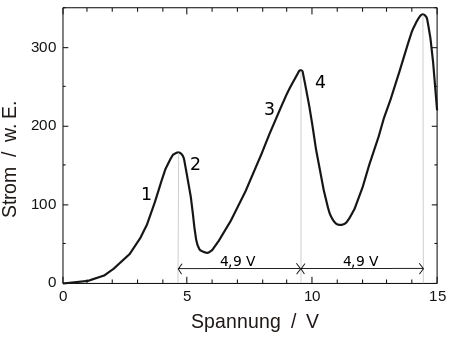
\includegraphics[width=\linewidth]{../figs/Franck-Hertz_spannungskurve}
        \caption{Franck-Hertz: Spannungskurve \cite{wiki:franck-hertz}}
        \label{fig:franck-hertz-spannungskurve}
    \end{minipage}
    \hspace{.5cm}
    \begin{minipage}{.45\linewidth}
        \centering
        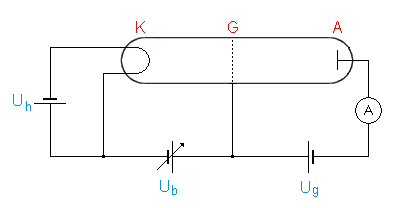
\includegraphics[width=\linewidth]{../figs/Schaltbild_Franck_Hertz_Versuch}
        \caption{Schaltbild Franck Hertz Versuche \cite{wiki:franck-hertz}}
        \label{fig:schaltbild_franck_hertz}
    \end{minipage}
\end{figure}

\subsection{Auswertung}
Die Unsicherheiten werden nach Herstellerangaben auf $\pm 1\%$ inklusive $\pm 0.5\%$ 
des Messbereiches gelegt. Der Messbereich beim genutzten Sensor ist variabel 
und wurde automatisch gesteuert, weshalb nur vermutet werden kann, dass dieser 
bei steigender Spannung immer auf den nächsten höheren Bereich umgestiegen ist. Die Fehler
wurden auf diese Weise für die Messung des Anodenstroms und Beschleunigungsspannung berechnet, wobei
zu beachten ist, dass kein eigentlicher Strom, sondern die dazu proportionale Spannung gemessen wurde.
Die Skalierung ist für die Auswertung jedoch nicht weiter wichtig. 

\begin{figure}[htb]
    \centering
    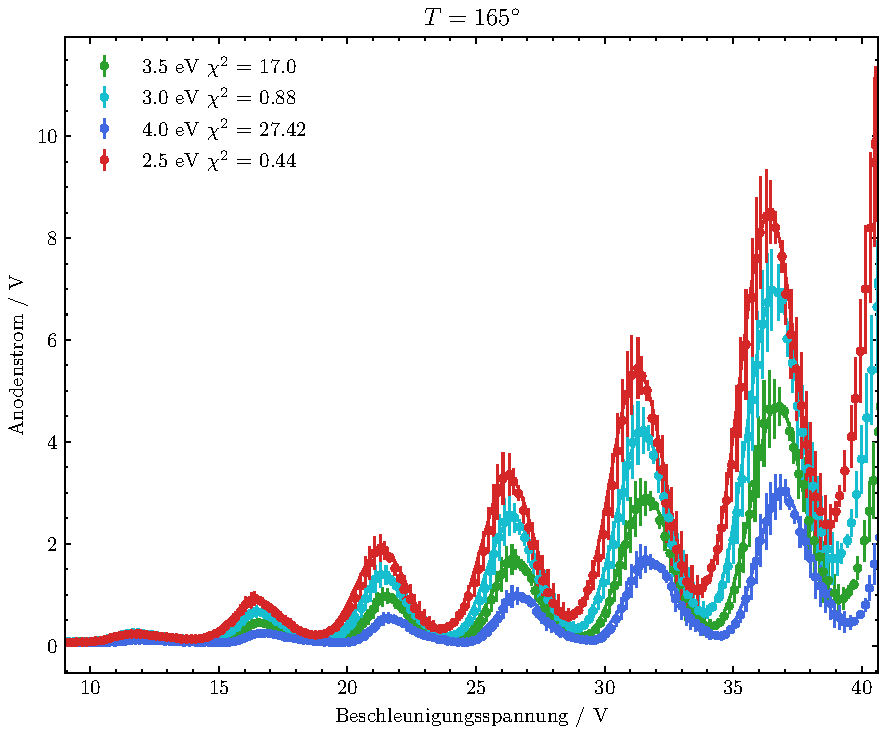
\includegraphics[width=0.6\linewidth]{../figs/franck-hertz_gegenspannung}
    \caption{Spannungskurve in Abhängigkeit der Gegenspannung bei \SI{165}{\celsius}}
    \label{fig:gegenspannung}
\end{figure}

\subsubsection{Abhängigkeit der Gegenspannung}\label{sec:franck-hertz-gegen}
Die Messdaten der Spannungskurven bei variabler Gegenspannung sind in 
\cref{fig:gegenspannung} grafisch dargestellt. An die Daten können Gauß-Kurven
angepasst werden. Die Parameter der Anpassung sind in \cref{tab:gegenspannung}
aufgezeigt. Das $\chi^2$ für die Anpassungen ist liegt dabei eine Größenordnung zu
hoch, da aber diese Maß der Güte nur die Fehler der y-Achse betrachtet und 
hier die Fehler in x-Richtung deutlich überwiegen, kann die Güte 
nicht die Anpassung richtig einschätzen. Visuell kann behauptet werden,
dass die Messdaten hier sehr gut beschrieben werden.

Zu Sehen ist, dass für größere Gegenspannungen 
die Maxima kleiner werden und leicht zu höheren Spannungen verschoben werden. 
Dies entspricht der Erwartung, dass bei höheren Gegenspannungen weniger 
Elektronen in den Bereich hinter das Gitter driften können.

Die Breite der Kurven nimmt dabei leicht ab, was jedoch im Fehlerbereich liegt.

Für Alle Gegenspannungen liegt die durchschnittliche Übergangsenergie im $1\sigma$-Bereich 
zum Literaturwert des Übergangs.

\subsubsection{Abhängigkeit der Temperatur}
Die Messdaten der Spannungskurven bei Variation der Temperatur 
sind in \cref{fig:temperatur} grafisch dargestellt und die Anpassparameter 
tabellarisch in \cref{tab:temperatur}. Die Güte der Anpassungskurven ist 
vergleichbar wie in \cref{sec:franck-hertz-gegen}. Auch hier ist erkennbar, dass 
bei steigender Temperatur die Maxima leicht zu höheren Spannungen hin verschoben 
werden mit gedämpften Amplituden und leicht erhöhten Breiten. Nach \cite{skript}
ist die Temperatur durch die Relation 
\begin{equation*}
    \log p = \num{10.55}-\frac{3333}{T}-\num{0.85}\log T
\end{equation*}
mit dem Druck korreliert. Diese Korrelation ist in \cref{fig:druck_temp} dargestellt. Wie zu 
erkennen ist, variiert in dem Bereich über der Raumtemperatur der Druck stark. Mit 
höherem Druck nimm ebenso die Anzahl der Stöße zu, weshalb weniger Elektronen die Gegenspannung
überwinden können und dadurch die Amplitude der Kurven sinkt. Die Driftgeschwindigket 
der Elektronen ist antiproportional zur freien Weglänge, weshalb bei erhöhter Temperatur 
eine höhere Beschleunigungsspannung zur Stoßanregung benötigt wird. Dies erklärt auch 
die leichte Verschiebung der Maxima. Zu Erkennen ist ebenfalls, dass für die ersten 
vier Maxima die Breite leicht zunimmt (bei dem ersten ist die Zunahme wieder sehr stark), 
für die letzten Beiden jedoch konstant bleibt. 
Eine offensichtliche Erklärung hierfür lässt sich nicht eindeutig finden. Es besteht 
die Möglichkeit, dass für zu kleine Spannungen die Energie der Elektronen sich in
dem Bereich befindet, wo nach \cref{fig:wirkungsquerschnitte} die Wirkungsquerschnitte
der zwei niedrigsten Übergänge ähnlich groß sind, weshalb sich hier die 
Kurven der Anregung überlagern.

Die Energien der Übergänge sind in \cref{tab:temperatur} aufgetragen mit dem Mittelwert 
in der letzten Spalte. Zu Erkennen ist dabei, dass bei der kleinsten Temperatur noch eine 
Energie von \SI{4.8(3)}{\electronvolt} gemessen wurde, bei höheren Temperaturen 
sinkt diese auf \SI{4.6(3)}{\electronvolt} ab. Dies lässt sich mit \cref{fig:wirkungsquerschnitte}
erklären. Bei zu hohen Temperaturen wird die freie Weglänge der Elektronen so stark begrenzt, 
dass nur noch das niedrigste Energieniveau angeregt werden kann. Bei zu kleinen Temperaturen 
würde hingegen der Übergang $6^1\mathrm S_0\rightarrow 6^1\mathrm P_1$ überwiegen. Der Bereich,
in dem der Streuquerschnitt des hier untersuchten Übergangs überwiegt, ist klein, weshalb 
das Temperaturintervall ebenso klein gewählt werden musste.

\begin{figure}[htb]
    \centering
    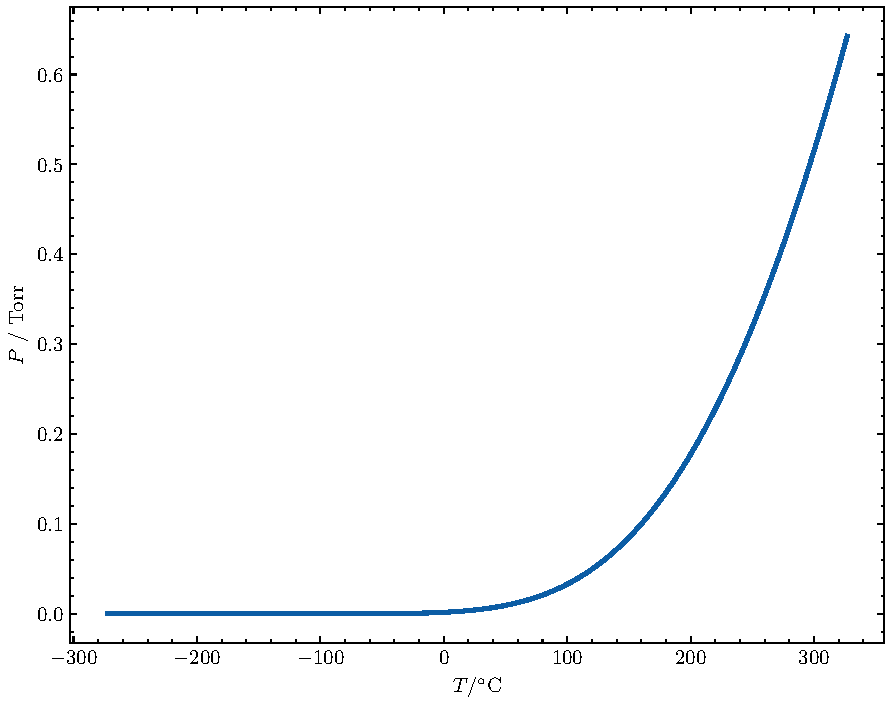
\includegraphics[width=.5\linewidth]{../figs/druck_temp}
    \caption{Temperaturabhängigkeit des Drucks}
    \label{fig:druck_temp}
\end{figure}


\begin{figure}[htb]
    \centering
    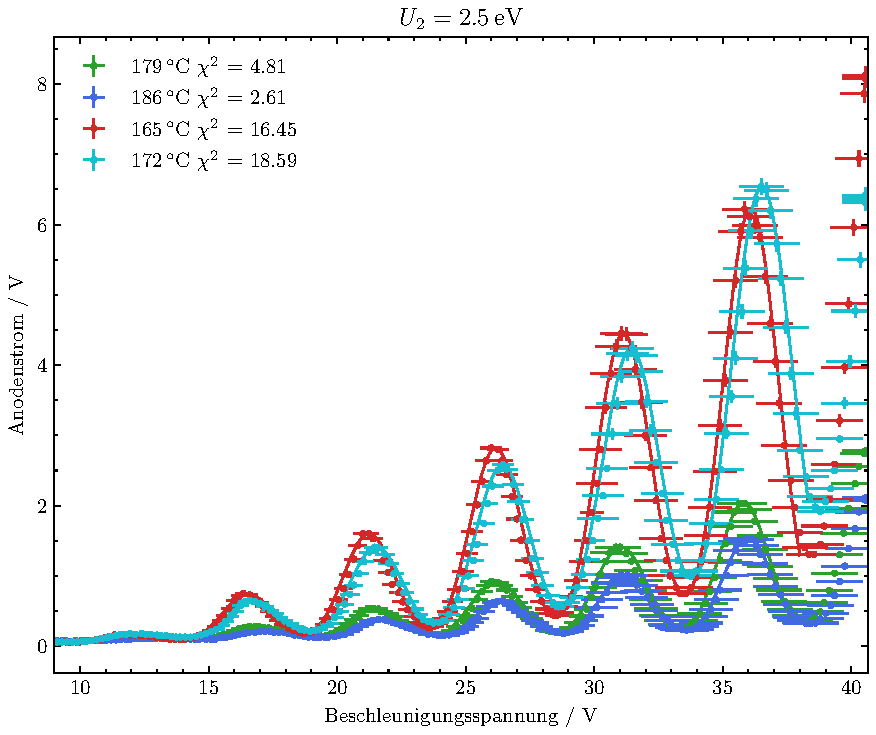
\includegraphics[width=0.6\linewidth]{../figs/franck-hertz_temperatur}
    \caption{Spannungskurve in Abhängigkeit der Temperatur bei einer Gegenspannung von \SI{2.5}{\volt}}
    \label{fig:temperatur}
\end{figure}

\begin{table}[htb]
   \centering
\caption{Anpassparameter der Spannungskurve für verschiedene Gegenspannungen}
\begin{tabular}{c|cc|cc|cc|cc}
\hline & \multicolumn{2}{|c}{\SI{2.5}{\volt}} & \multicolumn{2}{|c}{\SI{3.0}{\volt}} & \multicolumn{2}{|c}{\SI{3.5}{\volt}} & \multicolumn{2}{|c}{\SI{4.0}{\volt}}\\

\hline
Maximum & $x_0$ / \unit{\volt} & $\sigma$ / \unit{\volt} & $x_0$ / \unit{\volt} & $\sigma$ / \unit{\volt} & $x_0$ / \unit{\volt} & $\sigma$ / \unit{\volt} & $x_0$ / \unit{\volt} & $\sigma$ / \unit{\volt} \\ 
\hline
$\num{1}$ & $\num{11.97\pm 0.03}$ & $\num{1.35\pm 0.03}$ & $\num{11.96\pm 0.03}$ & $\num{1.28\pm 0.03}$ & $\num{12.10\pm 0.04}$ & $\num{1.49\pm 0.05}$ & $\num{12.17\pm 0.07}$ & $\num{1.84\pm 0.11}$ \\
$\num{2}$ & $\num{16.52\pm 0.03}$ & $\num{1.031\pm 0.016}$ & $\num{16.64\pm 0.03}$ & $\num{1.00\pm 0.02}$ & $\num{16.81\pm 0.04}$ & $\num{0.98\pm 0.03}$ & $\num{17.04\pm 0.05}$ & $\num{1.01\pm 0.04}$ \\
$\num{3}$ & $\num{21.32\pm 0.03}$ & $\num{1.023\pm 0.016}$ & $\num{21.47\pm 0.03}$ & $\num{0.999\pm 0.018}$ & $\num{21.61\pm 0.04}$ & $\num{0.96\pm 0.03}$ & $\num{21.77\pm 0.04}$ & $\num{0.96\pm 0.03}$ \\
$\num{4}$ & $\num{26.26\pm 0.03}$ & $\num{1.031\pm 0.019}$ & $\num{26.45\pm 0.03}$ & $\num{0.995\pm 0.019}$ & $\num{26.56\pm 0.04}$ & $\num{0.97\pm 0.03}$ & $\num{26.74\pm 0.05}$ & $\num{0.97\pm 0.03}$ \\
$\num{5}$ & $\num{31.29\pm 0.05}$ & $\num{1.10\pm 0.03}$ & $\num{31.50\pm 0.06}$ & $\num{1.04\pm 0.04}$ & $\num{31.66\pm 0.07}$ & $\num{1.02\pm 0.04}$ & $\num{31.85\pm 0.08}$ & $\num{0.97\pm 0.05}$ \\
$\num{6}$ & $\num{36.40\pm 0.07}$ & $\num{1.15\pm 0.06}$ & $\num{36.61\pm 0.09}$ & $\num{1.09\pm 0.06}$ & $\num{36.72\pm 0.11}$ & $\num{1.03\pm 0.07}$ & $\num{36.92\pm 0.13}$ & $\num{0.97\pm 0.09}$ \\
\hline\end{tabular}
\label{tab:gegenspannung}
\end{table}\begin{table}[htb]
   \centering
\caption{Anpassparameter der Spannungskurve für verschiedene Temperaturen}
\begin{tabular}{c|cc|cc|cc|cc}
\hline & \multicolumn{2}{|c}{\SI{165}{\celsius}} & \multicolumn{2}{|c}{\SI{172}{\celsius}} & \multicolumn{2}{|c}{\SI{179}{\celsius}} & \multicolumn{2}{|c}{\SI{186}{\celsius}}\\

\hline
Maximum & $x_0$ / \unit{\volt} & $\sigma$ / \unit{\volt} & $x_0$ / \unit{\volt} & $\sigma$ / \unit{\volt} & $x_0$ / \unit{\volt} & $\sigma$ / \unit{\volt} & $x_0$ / \unit{\volt} & $\sigma$ / \unit{\volt} \\ 
\hline
$\num{1}$ & $\num{12.00\pm 0.03}$ & $\num{1.43\pm 0.04}$ & $\num{12.33\pm 0.04}$ & $\num{1.57\pm 0.04}$ & $\num{12.42\pm 0.06}$ & $\num{1.99\pm 0.08}$ & $\num{12.79\pm 0.12}$ & $\num{3.0\pm 0.3}$ \\
$\num{2}$ & $\num{16.55\pm 0.03}$ & $\num{1.023\pm 0.016}$ & $\num{16.82\pm 0.03}$ & $\num{1.109\pm 0.018}$ & $\num{17.05\pm 0.03}$ & $\num{1.21\pm 0.03}$ & $\num{17.48\pm 0.04}$ & $\num{1.21\pm 0.05}$ \\
$\num{3}$ & $\num{21.24\pm 0.03}$ & $\num{1.030\pm 0.014}$ & $\num{21.53\pm 0.03}$ & $\num{1.094\pm 0.016}$ & $\num{21.51\pm 0.03}$ & $\num{1.15\pm 0.02}$ & $\num{21.80\pm 0.03}$ & $\num{1.25\pm 0.03}$ \\
$\num{4}$ & $\num{26.17\pm 0.03}$ & $\num{1.021\pm 0.016}$ & $\num{26.43\pm 0.03}$ & $\num{1.083\pm 0.016}$ & $\num{26.21\pm 0.03}$ & $\num{1.085\pm 0.017}$ & $\num{26.45\pm 0.03}$ & $\num{1.16\pm 0.02}$ \\
$\num{5}$ & $\num{31.15\pm 0.05}$ & $\num{1.06\pm 0.03}$ & $\num{31.43\pm 0.05}$ & $\num{1.14\pm 0.03}$ & $\num{31.04\pm 0.05}$ & $\num{1.06\pm 0.03}$ & $\num{31.24\pm 0.04}$ & $\num{1.11\pm 0.03}$ \\
$\num{6}$ & $\num{36.09\pm 0.06}$ & $\num{1.08\pm 0.04}$ & $\num{36.52\pm 0.07}$ & $\num{1.19\pm 0.05}$ & $\num{35.82\pm 0.06}$ & $\num{1.01\pm 0.05}$ & $\num{35.98\pm 0.07}$ & $\num{1.03\pm 0.05}$ \\
\hline\end{tabular}
\label{tab:temperatur}
\end{table}

\begin{table}[htb]
   \centering
\caption{Übergangsenergien bei verschiedenen Gegenspannungen}
\begin{tabular}{c c c c c}
\hline Maximum & \SI{2.5}{\volt} & \SI{3.0}{\volt} & \SI{3.5}{\volt} & \SI{4.0}{\volt} \\ 
\hline
$\num{1}$ & $\num{4.55\pm 0.04}$ & $\num{4.68\pm 0.04}$ & $\num{4.71\pm 0.05}$ & $\num{4.88\pm 0.09}$ \\
$\num{2}$ & $\num{4.80\pm 0.04}$ & $\num{4.83\pm 0.04}$ & $\num{4.79\pm 0.05}$ & $\num{4.73\pm 0.06}$ \\
$\num{3}$ & $\num{4.94\pm 0.04}$ & $\num{4.98\pm 0.05}$ & $\num{4.96\pm 0.06}$ & $\num{4.97\pm 0.06}$ \\
$\num{4}$ & $\num{5.03\pm 0.06}$ & $\num{5.05\pm 0.07}$ & $\num{5.10\pm 0.08}$ & $\num{5.11\pm 0.09}$ \\
$\num{5}$ & $\num{5.12\pm 0.09}$ & $\num{5.12\pm 0.11}$ & $\num{5.06\pm 0.13}$ & $\num{5.07\pm 0.15}$ \\
$\langle E\rangle$ & $\num{4.9\pm 0.3}$ & $\num{4.9\pm 0.3}$ & $\num{4.9\pm 0.3}$ & $\num{5.0\pm 0.3}$ \\
\hline\end{tabular}
\label{fig:energy_gegen}
\end{table}\begin{table}[htb]
   \centering
\caption{Übergangsenergien bei verschiedenen Temperaturen}
\begin{tabular}{c c c c c}
\hline Maximum & \SI{165}{\celsius} & \SI{172}{\celsius} & \SI{179}{\celsius} & \SI{186}{\celsius} \\ 
\hline
$\num{1}$ & $\num{4.54\pm 0.04}$ & $\num{4.50\pm 0.04}$ & $\num{4.63\pm 0.06}$ & $\num{4.69\pm 0.13}$ \\
$\num{2}$ & $\num{4.70\pm 0.03}$ & $\num{4.70\pm 0.04}$ & $\num{4.46\pm 0.04}$ & $\num{4.32\pm 0.04}$ \\
$\num{3}$ & $\num{4.93\pm 0.04}$ & $\num{4.91\pm 0.04}$ & $\num{4.70\pm 0.04}$ & $\num{4.65\pm 0.04}$ \\
$\num{4}$ & $\num{4.98\pm 0.05}$ & $\num{5.00\pm 0.05}$ & $\num{4.82\pm 0.05}$ & $\num{4.79\pm 0.05}$ \\
$\num{5}$ & $\num{4.95\pm 0.08}$ & $\num{5.09\pm 0.08}$ & $\num{4.78\pm 0.08}$ & $\num{4.73\pm 0.08}$ \\
$\langle E\rangle$ & $\num{4.8\pm 0.3}$ & $\num{4.8\pm 0.3}$ & $\num{4.7\pm 0.2}$ & $\num{4.6\pm 0.3}$ \\
\hline\end{tabular}
\label{fig:energy_temp}
\end{table}



% "Fazit"
\section{Fazit}\label{sec:fazit}
Mithilfe der Bragg-Reflexion konnte von zwei unterschiedlichen Anoden einer 
Röntgenröhre die K$_\alpha$ und K$_\beta$ Linien der charakteristischen 
Röntenstrahlung untersucht werden. Die Wellenlängen multipliziert mit der Beugungsordnung 
der Anode aus einem zuvor unbekannten Element sind in \cref{tab:anode-unbekannt}
vorzufinden. Dabei konnte festgestellt werden, dass sämtliche 
Linien Vielfache der ersten beiden Linien (vom Diagramm aus links gesehen)
darstellen, womit schlussgefolgert werden kann, dass die hier beobachteten Linien
zwei charakeristische Linien bis zur vierten Beugungsordnung darstellen solllen.
Das unbekannte Element konnte als Silber identifiziert werden, da 
dessen Spektrum eine K$_\beta$-Linie bei \SI{49.3}{\pm} aufweist und der 
Messwert von \SI{49.26\pm0.06}{\pm} im $1\sigma$-Bereich der Messung liegt. Eine K$_\alpha$ 
Linie liegt bei \SI{55.942}{\pm}, während eine Wellenlänge von \SI{55.63\pm0.05}{\pm}
gemessen werden konnte. Da die erste Linie mit der Literatur übereinstimmt, ist eine 
Abweichung bei der zweiten Linien ungewöhnlich. Eine Verschiebung 
des Kristalls während der Messung könnte Ursache für die Diskrepanz sein.\par 
Von einer Molybdän-Anode wurde zusätzlich die Feinstrukturaufspaltung 
der K$_\alpha$-Linie in der vierten Beugungsordnung gemessen, was in \cref{fig:feinstruktur}
zu sehen ist. In \cref{tab:feinstruktur} sind die gemessenen 
Energien im Vergleich zu den Literaturwerten zu sehen. Dabei konnte die Feinstrukturaufspaltung
auf drei signifikante Stellen genau gemessen werden, da jedoch die in diesem Versuch 
abgeschätzten Fehler deutlich kleiner sind, liegen die Referenzwerte nicht im $3\sigma$-Bereich
der Messung. Dies ist auch für Wellenlängendifferenz
\begin{equation*}
	\Delta\lambda_\mathrm{Exp} = \SI{0.444\pm 0.008}{\pm},\qquad
	\Delta\lambda_\mathrm{Ref} = \SI{0.428\pm0.004}{\pm}
\end{equation*}
zu beobachten, weshalb ein systematischer Fehler als Ursache für die Abweichung 
ausgeschlossen wird. Eine leichte Verschiebung des Kristalls stellt dabei 
eine realistische Fehlerquelle dar.\\\par

Mit der Röntgenfluoreszenz konnte die Zusammensetzung von 
Legierungen analysiert werden. Hierfür wurden mit verschiedenen metallischen Plätchen 
das dazugehörige Röntegenspektrum durch Fluoreszenz gemessen werden. Nach Kallibration
der Messung durch den Vielkanalanalysator konnte dem Spektrum Energien zugegeordnet werden und die 
Intensitäten der Linien konnten mit den Intensitäten der Legierungen verglichen werden und somit
die Massenanteile der Elemente. Hierbei konnte die zweite Legierung als 
Mischung von Kupfer und Zink identifiziert werden mit, im Fehlerbereich, gleichen Anteilen von 
\begin{equation*}
    C_\mathrm{Cu} = 49.6(5)\%,\quad C_\mathrm{Zn} = 50(2)\%.
\end{equation*}
Einen Vergleichswert hierzu gibt es nicht, weshalb eine quantitative Einordnung der Messwerte 
nicht möglich ist. Der Wert liegt jedoch in realistischen Bereichen.
\\\par

Im dritten Versuchsteil wurde die Symmetrie und Gitterstruktur eines NaCl-Kristalls mithilfe des Laue-Verfahrens
untersucht. Dazu wurde der zu untersuchende NaCl-Kristall über \SI{1800}{\second} mit von einer
Molybdän-Röntgenröhre erzeugten Röntgenstrahlung belichtet. Die Röntgenstrahlung wird teilweilse durch den
NaCl-Kristall transmittiert und teilweise an den unterschiedlichen Netzebenenscharen gebeugt. Hinter dem Kristall
wird die transmittierte und gebeugte Röntgenstrahlung mithilfe eines Röntgenfilms nachgewiesen, welcher nach
einer Entwicklung zur Auswertung bereit steht.\par
Ziel der Auswertung war es, die einzelnen Reflexe auf dem Röntgenfilm mit den entsprechenden Millerschen Indizes
zu identifizieren, welche die Orientierung der einzelnen Netzebenenscharen beschreiben. So konnte rausgefunden werden,
welche Netzebenenscharen des NaCl-Kristalls für welchen Reflex verantwortlich waren. Die Zuordnung der Millerschen
Indizes stellte hier eine Herausforderung da, da das Reflexmuster auf dem Röntgenfilm gewölbt war. Dennoch konnte
die Zuordnung unter Berücksichtung der Symmetrie des NaCl-Kristalls (kubische Symmetrie) erfolgreich durchgeführt werden.
Die Ergebnisse sind in \cref{tab:miller2} zu finden.\par
Anschließend konnten mit den Millerschen Indizes der Netzebenenabstand der einzelnen Netzebenen einer Netzebenenschar,
der Glanzwinkel und die für einen Reflex verantwortlichen Wellenlängen (es tragen mehrere Beugungsordnungen bei)
bestimmt werden. Die berechneten Werte sind in \cref{tab:keineahnung} einzusehen.

% "Anhang"
\appendix
\section*{Anhang}\label{sec:anhang}



% Literaturverzeichnis ausgeben
\printbibliography[heading=bibintoc, title = {Literaturverzeichnis}]

\end{document}
%========================================================================